\section{MOS}
Mi interessa studiare due fenomeni disgiunti l'uno dall'altro.
\begin{itemize}
    \item controllo e accumulo di carica per effetto di induzione elettrostatica;
    \item trasporto di carica grazie a un campo elettrico.
\end{itemize} 
Prima di tutto si parte con il costruire un MOS:
Si prende un semiconduttore di tipo p con un'estremità collegata a ground e sull'altra estremità faccio crescere dell'ossido, tipicamente SiO2, che serve per separare il semiconduttore dal metallo posto successivamente. Il metallo rappresenta il "gate" ed è collegato al potenziale $V_G$. \\
PS: molto della tecnologia MOS si basa sul biossido di Silicio.\\

La struttura ideale del mos prevede che Metallo e semiconduttore siano scelti in modo che il loro lavoro di estrazione sia identico ($E_{WM}=E_{WSC}$)
comportando l'assenza di passaggi (prima era scritto sbagliato = accumuli) di carica quando non si applica un potenziale.
Questo fenomeno è ottenuto grazie al fatto che tra i due è interposto un ossido (tipicamente SiO2) con ampiezza della banda proibita molto alta impedendo il passaggio di portatori dal metallo al semiconduttore. questo schema prende il nome di banda piatta, termine derivante dal livello di vuoto con andamento piatto (caso assenza di polarizzazione).

 \begin{figure}[h]\centering
    \subcaptionbox{BJT npn con modello a diodi}[.4\linewidth][c]{%
    
\includegraphics[]{ImmaginiMOS/MOS.png}
    }
\hfil  
\subcaptionbox{BJT npn}[.4\linewidth][c]{%
    
\includegraphics[]{ImmaginiMOS/MOS-diagrammaBande.png}
}
\label{MOS}
\end{figure}

\subsection{Accumulo di carica - il condensatore MOS}

%Si può immaginare il MOS come una struttura che accumula elettroni.\\
%Esistono gli n-MOS e p-MOS, ovvero strutture che accumulano elettroni oppure lacune.
%Un n-MOS accumula elettroni in un canale di tipo n. \\

Abbiamo assodato quindi che i passaggi di carica sono interdetti a causa dell'ossido che si trova in mezzo, tuttavia può verificarsi un accumulo di carica per induzione elettrostatica.
L'accumulo di carica è sinonimo di condensatore.\\
in totale possiamo considerare tre condizioni di funzionamento
\begin{itemize}
    \item $V_G=0$: ai capi della giunzione non è presente alcuna tensione di built-in. Siamo nel caso ideale di banda piatta (se vale la condizione di equilibrio termodinamico);
    \item $V_G>0$: Stato di accumulo di lacune;
    \item $V_G<0$: Stato di accumulo di elettroni (detto anche svuotamento di lacune).
\end{itemize}
%
\cleardoublepage
\subsubsection{Stato di accumulo di lacune $(V_G < 0)$} pg488
Applicando una tensione negativa sul metallo e positiva sul semiconduttore si instaura un campo elettrico diretto verso il metallo.\\
In questa situazione gli elettroni del metallo verranno spinti nella direzione opposta al capo elettrico, dirigendosi verso la superficie di contatto metallo-ossido. Il ragionamento è duale per le lacune: vengono spinte con verso concorde al campo elettrico fino ad arrivare all'interfaccia ossido-semiconduttore.

Osserando l'andamento della distribuzione di carica in questa struttura vedo due delta di dirac, una positiva e una negativa.
\begin{figure}[hbt!]
    \centering
    
\includegraphics[width=0.55\textwidth]{ImmaginiMOS/MOS-Vgmin0.png}
    \caption{Caption}%
    \label{fig:enter-label}
\end{figure}
%
\begin{psbox}
il livello di fermi del SC rappresenta il livello massimo oltre il quale non ci sono elettroni legati con legami covalenti.
In un semiconduttore p il livello di fermi è vicino alla banda di valenza perchè stò drogando il SC-i con atomi del quarto quadrante con il conseguente eccesso di lacune (e diminuzione di elettroni).

Se nel SC-p inserisco una tensione positiva, e quindi ulteriori lacune, i pochi elettroni nella banda di conduzione si accoppieranno con le lacune.
gli elett liberi diminuiscono e quindi anche il livello di fermi
\end{psbox}

In questa situazione succederà che l'accumulo di lacune nel semiconduttore farà abbassare il livello di Fermi di quest'ultimo. ecco spiegato la curvatura della banda senza la presenza di regione di svuotamento
\begin{ricevimento}
    ???
\end{ricevimento}

\begin{comment}
\begin{exbox}[valutare se tenere]
Le lacune presenti nella regione "p" sono attratte verso la superficie del ossido-semiconduttore perché vengono attratte dalle cariche negative causate dalla tensione applicata al metallo.
Allo stesso tempo, poiché le lacune si accumulano sulla superficie del semiconduttore, si verifica anche un accumulo superficiale di elettroni dalla parte del metallo. 
\end{exbox}
\end{comment}


\begin{ricevimento}
    cosa c'èntra che le lacune sono maggioritari sul p? e debye?
\end{ricevimento}

poiché lo spessore della sezione di cariche negative e positive formatasi è minore della lunghezza di Debye, si può approssimare che la maggior parte della differenza di potenziale tra il metallo e il semiconduttore si verifica attraverso lo strato di ossido che separa il metallo dal semiconduttore. Questo accade a causa delle caratteristiche elettriche dell'ossido, come la sua maggiore resistività rispetto al metallo e al semiconduttore.
Ipotizzando un ossido ideale (completamente isolante cioè priva di cariche al suo interno), l'assenza di carica implica che il campo elettrico è costante da cui si ottiene l'energia potenziale con andamento lineare.

\begin{exbox}[da chatgpt]
    Dell'ordine della lunghezza di Debye nei due materiali": La lunghezza di Debye è una misura della distanza su cui le cariche in un materiale si schermano reciprocamente a causa delle interazioni coulombiane. Quando si dice che lo spessore degli strati di cariche è "dell'ordine della lunghezza di Debye", significa che sono molto sottili e che le interazioni coulombiane tra le cariche si estendono solo su distanze molto brevi, come approssimativamente la lunghezza di Debye nei due materiali coinvolti.
\end{exbox}

L'ossido si comporta come una quasi-capacità, supponendo che la mobilità dei portatori maggioritari in P sia elevata (sicuramente c'entra con debye).\\
Il valore della capacità che fornisce l'ossido è : 
\begin{equation}
    C_{ox}=\dfrac{\varepsilon_{ox}}{t_{ox}}
\end{equation}
Dove $t_{ox}$ è la larghezza dell'ossido e $\varepsilon_{ox}$, la costante dielettrica dell'ossido.

pertanto la carica superficiale accumulata nel semiconduttore vale
\begin{equation}
    Q_t=C_{ox}V_G
\end{equation}
mentre la carica superficiale accumulata nel metallo sarà $Q=-Q_t$.


\cleardoublepage
\subsubsection{Stato di svuotamento di lacune $(V_G > 0)$}

\begin{figure}[h]
    \centering
    
\includegraphics{ImmaginiMOS/MOS-Vgmag0.png}
    \caption{Caption}%%
    \label{fig:enter-label}
\end{figure}

Applicando al metallo un potenziale positivo $Vg > 0$ il semiconduttore si riempie di elettroni e di conseguenza si ha un aumento del livello di fermi. nel diagramma a bande il SC va verso l'alto.\\
Siccome il metallo stà venendo caricato positivamente, le lacune presenti nel semiconduttore si allontanano dalla zona vicino al metallo, facendo abbassare la concentrazione di lacune all'interfaccia ossido-semiconduttore, creando una sorta di regione di svuotamento come visto nel caso PN.
\begin{ricevimento}[non ha senso?]
chiedere se quello sopra è giusto
\end{ricevimento}

La densità di carica nel lato del metallo è come nel caso precedente. la sola differenza è il segno positivo.\\
la carica superficiale $Q_d$ presente nel lato del metallo dovrà essere uguale ed opposta alla carica di giunzione prensente della regione di svuotamento (di lunghezza d) nel lato semiconduttore $-Q_d$.
La carica superficiale all'interno della giunzione sarà pari a $-\rho \cdot d = -q\cdot N_A \cdot d$ quindi la carica nel metallo sarà il suo opposto:
\begin{equation}
    Q_d=q N_A d
\end{equation}
\begin{ricevimento}
    è una carica superficiale? $Q_d=rho *d$, manca l'area
\end{ricevimento}
$d$ è lo spessore della regione di svuotamento.\\
Ora il mio scopo è cercare di ricavare il potenziale totale di questo dipositivo. per fare questo mi servirà conoscere quanto vale il potenziale lungo l'ossido ($\phi_{ox}$) e quello lungo il semiconduttore ($\phi_{s}$). Per continuare devo fare un richiamo dell'equazione di Poisson applicato ad un sistema di riferimento che parte dal lato sinistro dell'ossido (x=0) e si dirige verso il semiconduttore per $x>0$ (idealmente fino ad $\infty$) :
%
\begin{equation}
    \dfrac{d^2\phi(x)}{dx^2}=\dfrac{-\rho}{\varepsilon}
\end{equation}
%
Quindi prendo Poisson e lo integro una prima volta:
%
\begin{equation}
    \dfrac{d \phi(x)}{dx}=-\dfrac{qN_Ad}{\varepsilon}x +A
\end{equation}
%
Per trovare $\phi(x)$ lo integro una seconda volta:
%
\begin{equation}
    \phi(x)=-\dfrac{1}{2}\left(\dfrac{qN_Ad}{\varepsilon}\right)x^2 +Ax + B
\end{equation}
%
Per calcolare le incognite A e B, devo considerare le condizioni al contorno.
%
\begin{ricevimento}
    serve una mano per risolvere poisson qui
    \begin{enumerate}
        \item lungo l'ossido non c'è carica. il campo elettrico è costante
        \item ad infinito, o cmq dopo x=d il campo elettrico è nullo ed il potenziale è massimo pari a $-qV_G$ (senza considerare tensioni di built in)
    \end{enumerate}
    \begin{center}
        \begin{tikzpicture}[scale=0.5]
             %disegno asse x
            \draw [->](-2,0)node[anchor=north]{}--(5+2,0)
            node[anchor=west]{$x$};
            %disegno asse y
            \draw [->](0,-3.5)--(0,3+1.5)node[anchor=south west]{$\rho_{fissa}(x)$};
            %disegno grafici
            \draw [thick,pattern=north east lines, pattern color=gray](2,0)rectangle++(4,-2);
            \draw [-latex, line width=0.75mm] (0,0)--++(0,+3)node[left]{$qN_Ad$};
            \draw[dashed](2,2)--++(0,-19);
            %label
            \node at (2,0) [above]{$t_{ox}$};
            \node at (2+4,0) [above]{$t_{ox}+d$};
            \node at (2+2,-1) [red]{$Q_d$};

            %disegno grafico energia
            %disegno asse x
            \draw [->](-2,-7.5)node[anchor=north]{}--(9,-7.5)
            node[anchor=west]{$x$};
            %disegno asse y
            \draw [->](0,-9.5)--(0,-3.7)node[anchor= west]{$\mathcal{E}(x)$};
            %disegno grafico rosso
            \draw [thick,red](0,-5)--(2,-5)--(6,-7.5)--++(1,0);
            %label
            \node at (0,-9) [anchor=west]{$\mathcal{E}_{MAX}$};

            %disegno grafico potenziale
            %disegno asse x
            \draw [->](-2,-12.5)node[anchor=north]{}--(6,-12.5)
            node[anchor=west]{$x$};
            %disegno asse y
            \draw [->](0,-15.5)--(0,-9.7)node[anchor= west]{$\phi(x)$};
           
            %disegno grafico potenziale
            \draw [thick](0,-12.5).. controls (1.5,-12.5) and (1,-15.7) ..(4,-15.5)--++(1,0);
            \draw[<->](4,-15.5)--(4,-12.5);
            \node at (4,-14)[anchor=west]{$q(V_{bi}-V_A)$};
            %label
            \node at (0,-11) [anchor=west]{$\mathcal{E}_{MAX}$};
    \end{tikzpicture}
    \end{center}
\end{ricevimento}
%
Definisco $x=t_{ox}$ il punto dopo finisce l'ossido (e $x=t{ox}+d$ il punto dove finisce la regione di svuotamento).\\

la caduta di potenziale sull'ossido si calcola risolvendo:
%
\begin{equation}
    \phi_{ox}= \phi(0)-\phi(t_{tox})=
\end{equation}
%
\\
trovo che:

\begin{equation}
    \Phi_{ox}=\dfrac{+qN_Ad\ t_{ox}}{\varepsilon_{ox}}
\end{equation}

\begin{exbox}
    Dato che gli spessori del metallo e SC sono fini, allora posso dire che il potenziale applicato all'ossido è uguale al potenziale applicato al solo condensatore MOS e varrà:
\begin{equation}
    \Phi_{ox}=\dfrac{Q_d}{C_{ox}}
\end{equation}
\end{exbox}

Per calcolare il potenziale sul semiconduttore devo considerare 
\begin{equation}
    \phi_{ox}= \phi(t_{ox})-\phi(\infty)=
\end{equation}
trovo
\begin{equation}
    \Phi_{sc}=\frac{q\ N_A\ d^2}{2\ \varepsilon_{SC}}
\end{equation}
Graficamente si avrà un andamento di questo genere:
\begin{figure}[hbt!]
    \centering
    
\includegraphics{ImmaginiMOS/MOS-PHI.png}
    \caption{Caption}%
    \label{fig:enter-label}
\end{figure}
Quindi se il livello del vuoto prima dell'applicazione del potenziale era piatto, ora avrà un incremento lineare dentro l'ossido e poi un andamento quadratico dentro il SC, dove quello lineare è dovuto a $\Phi_{ox}$, quello quadratico è dovuto a $\Phi_s$.\\
E' fondamentale capire che la somma dei potenziali (di ossido e SC) deve essere pari al potenziale $V_G$ applicato dalla batteria:
\begin{equation}
    V_G=\Phi_{ox}+\Phi_s   
\end{equation}
Questo mi permette di calcolare il rapporto tra lo spessore della regione svuotata e quello dell'ossido:

\begin{equation}
\dfrac{d}{t_{ox}}=\dfrac{\varepsilon{sc}}{\varepsilon_{ox}}+\sqrt{\dfrac{\varepsilon_{sc}^2}{\varepsilon_{ox}^2}+\dfrac{2\ V_G\ \varepsilon_{sc}}{q\ N_A\ t_{ox}^2}}
\end{equation}
Da questa equazione vedo che se $V_G>0$, allora lo spessore della regione di svuotamento aumenta con $V_G$.\\

\cleardoublepage
\subsubsection{Inversione di lacune per $V_G >> 0$}
Io sò che per $V_G>0$ si crea dalla parte del semiconduttore una regione di svuotamento dovuto ad elettroni attirati verso il metallo, pertanto il livello di fermi (intrinseco) in prossimità dell' ossido-semiconduttore tenderà ad abbassarsi perchè si riduce il numero di elettroni liberi di muoversi.

Se aumento la $V_g$ Il metallo viene riempito con altre cariche positive attirando sempre più gli elettroni nella parte del semiconduttore. Questo significa che nel SC ci saranno ancora meno elettroni liberi di muoversile e quindi il livello di fermi si abbassa ancora, arrivando al caso in cui concide con il livello di quasi fermi del semiconduttore ($E_{Fi}=E_{EFp}$).
Questo significa che il semiconduttore, all'interfaccia con l'ossido, non si comporta più come un SC-p ma come un SC intreinseco.\\
Posso spiegarlo anche matematicamente, partendo dall'equazione di Schockley :
%
\begin{equation}
    n(x) = n_i\ exp\left[\frac{E_F-E_{Fi}(x)}{K_BT}\right]
\end{equation}
Se $E_F=E_{Fi}$ allora troverò che $n(x)=n_i$.\\


Aumentando ancora di più la tensione ($V_G \gg 0$) succederà che il livello di fermi intrinseco scenderà sotto il livello di quasi fermi $E_Fp > E_{Fi}$.\\
Io sò che il caso in cui $E_F > E_{Fi}$ combacia con un SC drogato n pertanto, all'interfaccia ossido-SC, gli elettroni diventano portatori maggioritari. Si ha quello che si definisce "inversione di popolazione, nella quale il semiconduttore si comporta come fosse drogato n.
%
\begin{figure}[hbt!]
    \centering
    
\includegraphics{ImmaginiMOS/MOS-FERMI 1.png}
    \caption{Caption}%
    \label{fig:enter-label}
\end{figure}
%
Si ha una vera e propria inversione quando la concentrazione degli elettroni in $t_{ox}$ è uguale alla concentrazione dei droganti nel SC-p cioè lacune (e quando accade si avrà sicuramente che $E_{F}(tox)> E_{F}(t_ox)$). In questa particolare situazione si considera che $V_G$ abbia assunto il potenziale $V_{th}$.\\ 
$V_{th}$ viene intesa come soglia, ma cmq ci sono elettroni anche prima di raggiungere $V_{th}$, ecco perché alcuni MOS possono lavorare sotto soglia.\\
Si definisce la condizione di inversione di popolazione (che, ripeto, accade quando ):
%
\begin{align}
    n(t_{ox})&=N_A=p(+\infty)\\
    {V}_G&=V_{th}
\end{align}
%
In questa situazione vado a definire $\rho$, fra $t_{ox}$ e $t_{ox}+d$ e vedo che ha la solita concentrazione di ioni fissi negativi, ma all'interfaccia ossido-semiconduttore c'è anche una distribuzione di elettroni. Poi c'è un'altra carica all'interfaccia ossido-metallo.\\
\begin{ricevimento}
    non capito bene quelle righe sopra e sotto
\end{ricevimento}
Oltre alla carica fissa dovuta agli ioni del drogante si ha anche una carica mobile che si muove in un semiconduttore che originariamente era p, quindi pieno di ioni fissi negativi.

Dalle equazioni di Shotkley per un SC-p so che:
\begin{equation}
    p(x) =n_i\cdot exp\left[\frac{E_{Fi}(x)-E_F}{k_BT}\right]
\end{equation}
Se considero un punto x lontanissimo dalla giunzione con l'ossido ($x=\infty$) avrà $p(+\infty)\approx N_A$, perciò:
%
\begin{equation}
    N_A =n_i\cdot \exp{\left(\dfrac{E_{Fi}(\infty)-E_F}{k_BT}\right)}=n_i \exp{\left( \dfrac{\Phi_p}{V_T}\right)}
\end{equation}
Dove $\Phi_p=E_{Fi}(\infty)-E_F$, basta guardare le figure per capirlo 
\begin{ricevimento}
    leggere sopra. come lo potrei capire senza guardare le figure??
    $\Phi_p=E_{Fi}(\infty)-E_F$
\end{ricevimento}
%
Ora prendo l'equazione di Shotkley per gli elettroni:
%
\begin{equation}
    p(x) =n_i\cdot exp\left[\frac{E_{Fi}(x)-E_F}{k_BT}\right]
\end{equation}
%
Se considero il punto $x=t_{ox}$ avrò
%
\begin{align}
    n(t_{ox})&=n_i\cdot \exp{\left(\frac{E_F-E_{Fi}(t_{ox})}{k_BT}\right)}
\end{align}
Sapendo che alla tensione $V_G=V_{th}$ avviene l'inversione di popolazione, significa che $n(t_{ox})=p(+\infty)$ da cui ottengo:
\begin{align}
    E_F-E_{Fi}(t_{ox})=q\Phi_p
\end{align}
Con $\Phi_p=V_T\ log\left(\frac{N_A}{n_i}\right)$.

Pertanto la caduta di potenziale totale sul semiconduttore vale:
\begin{equation}
    \Phi_s=\dfrac{E_{Fi}(\infty)-E_{Fi}(t_{ox})}{q}=\dfrac{[\overbrace{E_{Fi}(\infty)-E_{Fi}}^{+q\Phi_p}]- [\overbrace{E_{Fi}(t_{ox})-E_{Fi}}^{-q\Phi_p}]}{q}=2 \Phi_p
\end{equation}

\begin{figure}[hbt!]
    \centering
    
\includegraphics{ImmaginiMOS/MOS-PHI2.png}
    \caption{Caption}%
    \label{fig:enter-label}
\end{figure}

La distanza fra $E_F$ e $E_{Fi}$ dipende dal drogaggio, sei all'inversione quando la distanza fra il livello di Fermi del semiconduttore e del metallo e il livello $E_{Fi}$ è uguale. La chiami $q\Phi_p$.
Eguagliando le due equazioni trovi l'innesco. $\Phi_p$ è dato dal drogaggio.
Quella carica è quella che ti serve per far funzionare il MOS.
Il potenziale applicato ad una struttura MOS implica una deformazione delle bande che comporta un'inversione della popolazione che da p diventa n. Questo accumulo è localizzato nei pressi della giunzione ossido-semiconduttore. La densità di carica $\rho$ prevederà sia carica fissa che mobile, dato che è un condensatore ci sarà carica uguale, ma di segno opposto all'altra interfaccia.

\subsection{Calcolo del potenziale di giunzione}
Ora voglio sapere a quale potenziale si innesca il fenomeno di inversione.\\
Parto cercando di calcolare la carica totale $Q_t$ che c'è all'interfaccia fra ossido e semiconduttore, ovvero a nella zona in cui è situato il canale. Essa sarà la somma di due cariche:
%
\begin{equation}
    Q_t=Q_n+Q_d
\end{equation}
%
Dove $Q_d$ è la carica dei portatori liberi presenti quando il canale è formato (quando scorre la corrente, la corrente è costituita da questi portatori);
$Q_n$ è la carica di giunzione, meglio definita come la carica immagazzinata nella regione di svuotamento.\\

Il valore della carica $Q_t$ può essere ricavata considerando il caso di un condensatore a facce piane e parallele alimentato da una tensione V. Dopo tutto il MOS si basa proprio su questo; L'ossido si comporta come un condensatore.\\
La differenza di potenziale che interessa alla capacità non è esattamente la $V_G$ infatti, devo sottrarre la tensione che cade nel semiconduttore per fare rimanere solo quella che interessa solo sull'ossido. Ricordando che $qV_G=q\Phi_s+q\Phi_{ox}$ ricavo che $\Phi_{ox}=V_G-\Phi_s$, allora:
\begin{align}
Q_t&={-C}_{ox}(\Phi_{ox})\\ \nonumber
    Q_t=Q_n+Q_d&={-C}_{ox}(V_G-\Phi_s)\\ 
Q_d&=-qN_A d
\end{align}
Ricordo che:
\begin{align}
{2\Phi}_p&=\frac{q\ N_A\ d^2}{2\ \varepsilon_{SC}}
\end{align}
%
\begin{ripasso}
Nel contesto di un transistor MOSFET di tipo P (PMOS), abbiamo una giunzione PN tra il substrato di tipo P e la regione di canale di tipo N. In presenza di una tensione applicata alla porta, si sviluppa una regione di svuotamento nel substrato di tipo P.

\(Q_d\) rappresenta la carica di svuotamento indotta dalla tensione applicata alla porta. \(q\) è la carica elementare (circa \(1.602 \times 10^{-19}\) Coulomb). \(N_A\) è la concentrazione di atomi accettori nel substrato di tipo P. \(d\) è la lunghezza della regione di svuotamento.

La relazione si ottiene attraverso l'equazione di Poisson, che lega il gradiente del potenziale elettrico alla densità di carica. L'equazione di Poisson per una giunzione PN in equilibrio può essere scritta come:
\[
\frac{d^2 \phi}{dx^2} = -\frac{q}{\varepsilon} (p - n + N_A^+ - N_D^-)
\]
Dove:
\begin{itemize}
    \item \(\phi\) è il potenziale elettrico.
    \item \(x\) è la coordinata spaziale nella direzione della giunzione.
    \item \(p\) e \(n\) sono le concentrazioni di portatori di carica di tipo P e N rispettivamente.
    \item \(N_A^+\) e \(N_D^-\) sono le densità di atomi accettori e donatori.
\end{itemize}

In una giunzione PN in equilibrio, il gradiente del potenziale è nullo, quindi:
\[
\frac{d^2 \phi}{dx^2} = 0
\]
In questo caso, la densità di carica nella regione di svuotamento è principalmente dovuta alla presenza di atomi accettori (\(N_A^+\)). La densità di carica negativa è data da:
\[
qN_A^+ = -qN_A
\]
Moltiplicando questa densità di carica per la lunghezza della regione di svuotamento \(d\), si ottiene la carica di svuotamento \(Q_d\):
\[
Q_d = -qN_A d
\]
Quindi, la relazione \(Q_d = -qN_A d\) riflette la carica di svuotamento nel substrato di tipo P di un transistor MOSFET di tipo P in equilibrio sotto l'effetto di una tensione applicata alla porta.

\end{ripasso}
%
alla fine troverò che
%
\begin{align}
    Q_d&=-\sqrt{2\ q\ \varepsilon_{SC}\ N_A\ 2\ \Phi_p}\\
Q_n=Q_t-Q_d&=-C_{ox}\left(V_G-2\ \Phi_p\right)+\sqrt{2\ q\ \varepsilon_{SC}\ N_A\ 2\ \Phi_p}
\end{align}
%
Per trovare la tensione di soglia oltre il quale si genera carica libera, dovrò considerare la situazione limite nel quale $V_G$ assume quell'ultimo valore (chiamato $V_{T0}$) per il quale la carica libera non si è ancora formata (è ancora nulla). In teoria sarebbe quando è $N_A$, c'è un po' di incongruenza nel ragionamento, per semplicità la poni uguale a 0. 
%
\begin{ricevimento}
    chiarite la frase precedente
\end{ricevimento}
%
Tale tensione è ottenuta manipolando le equazioni precedenti ponendo $Q_n=0$ e $V_G=V_{T0}$:
%
\begin{equation}
    V_{T0}=2\ \Phi_p+\frac{\sqrt{2\ q\ \varepsilon_{SC}\ N_A\ 2\ \Phi_p}}{C_{oX}}
\end{equation}
%
Ricordare che la tensione di soglia è il valore per il quale la carica libera ancora non c'è, ma inizia ad accumularsi. Dalla formula capisco che la soglia dipende dal valore di potenziale ai capi dell'ossido $\Phi_p=\Phi_s/2$ (ma anche da $\Phi_s$).
(in realtà Qn viene generata a partire dal valore di Na, ma questa è un'approssimazione)
%
\begin{ricevimento}
       non ho capito questa cosa tra parentesi
\end{ricevimento}
 %
L'accumulo di carica in un MOS è lineare. e scorre fra un ossido e un semiconduttore drogato p. l'ossido per sua natura è non conduttore perciò non è fatto per trasportare elettroni, in più il semiconduttore è drogato p, è una corrente molto impura. Da qui arrivo a dire che il trasporto di queste cariche non è molto efficiente (bassa corrente)
%
\cleardoublepage
%
\subsubsection{tensione di Bulk}
Tutti i ragionamenti fatti i precedenza si basano sull'assunzione che il Bulk (semiconduttore P+) sia collegato a massa, ma non è detto che sia così. Ci possono essere casi in cui il substrato non è a zero.

\begin{figure}[h]
    \centering
    
\includegraphics{ImmaginiMOS/MOS.png}
    \caption{Caption}%
    \label{fig:enter-label}
\end{figure}

Se la $V_B$ è potenzialmente diversa da zero tutto si depolarizza e l'espressione della tensione di soglia, adesso identificata come $V_{th}$ , si modifica di conseguenza:
\begin{equation}
    V_{th}=2\ \Phi_p+\frac{\sqrt{2\ q\ \varepsilon_{SC}\ N_A\ (2\ \Phi_p-V_B)}}{C_{oX}}
\end{equation}

La spiegazione è intuitiva. Adesso sull'ossido non ci cade solo il potenziale $\Phi_s$ ma anche $V_B$  permettendo di unare meno $V_G$ per innescare il meccanismo di creazione del canale.\\
\textbf{La tensione di soglia può cambiare in funzione della tensione di Bulk e questo è di fatto l'unico modo in cui può cambiare la tensione di soglia senza agire sul drogaggio o la $C_{ox}$.}\\
E' possibile riscrivere la $V_{th}$ attraverso $V_{t0}$
sostituisco la $Q_n$ all'interno del calcolo della corrente del canale del MOS. (??)

La Vt la puoi riscrivere in termini della Vt0:
\begin{align}
    V_T=V_{T0}+\gamma_B\left[\left(2\ \Phi_p-V_B\right)^{1/2}-\left(2\ \Phi_p\right)^{1/2}\right]
\end{align}
dove
$\gamma_B=\dfrac{\sqrt{2\ q\ \varepsilon_{SC}\ N_A\ }}{C_{oX}}$ prende il nome di  “Body factor”



\section*{9-11-2023}
\subsection{Non idealità legate alla struttura del MOS}
Le precedenti considerazioni sono state fatte sulla base di approssimazioni spinte che, in generale, non sono mai vere e dovranno essere rimosse per creare una formulazione più corretta.

\begin{enumerate}
    \item  Il lavoro di estrazione del metallo $E_{WM}$ e del semiconduttore $E_{WSC}$ non sono uguali.
    %%%
\begin{equation}
            E_{WM} \neq E_{WSC} = E_{WMS}
        \end{equation}
        \begin{center}
    \begin{tikzpicture}
        %disegno metallo
        \draw(0,1.25)node[left]{$E_{VMe}$}--(2,1.25); %livello fermi metallo
        \draw(0,2.75)node[left]{$E_{CMe}$}--(2,2.75); %disegno banda di conduzione metallo
        %disegno ossido
        \draw(2,-1)--(2,3);
        \draw(3,-1)--(3,3);
        %disegno semiconduttore
        \draw(3,-0.35)--(7,-0.35)node[right]{$E_{VSC}$}; %Ev SCp
        \draw(3,0)--(7,0)node[right]{$E_{F}$}; %lifello fermi SCp
        \draw (3,0.575)--(7,0.575)node[right]{$E_{Fi}$};%disegno fermi intrinseco
        \draw(3,1.5)--(7,1.5)node[right]{$E_{CSC}$}; %Ec SCp
        
    \end{tikzpicture}
\end{center}
\begin{center}
    \begin{tikzpicture}
        %disegno metallo
        \draw(0,1.25)--(2,1.25); %livello fermi metallo
        \draw(0,2.75)--(2,2.75); %disegno banda di conduzione metallo
        %disegno ossido
        \draw(2,-1)--(2,3);
        \draw(3,-1)--(3,3);
        %disegno semiconduttore
        \draw(3,-0.35)to [out=70, in=180](5,-0.35+1.25)--(7,-0.35+1.25); %Ev SCp
        \draw(3,0+1.25)--(7,0+1.25); %lifello fermi SCp
        \draw (3,0.575)to [out=70, in=180](5,0.575+1.25)--(7,0.575+1.25);%disegno fermi intrinseco
        \draw(3,1.75)to [out=70, in=180](5,1.5+1.25)--(7,1.5+1.25); %Ec SCp
        
    \end{tikzpicture}
\end{center}
%%%
Questo significa che a MOSFET spento, non si ha la naturale condizione di float band.la differenza nel lavoro di estrazione darà luogo ad una carica Qm già presente nel canale anche a MOSFET spento. Quindi, dato:\begin{equation}
    E_{WMe}-E_{WSCp}=E_{WMS}
\end{equation}
La carica nel canale sarà
\begin{equation}
    Q_{m}=C_{ox}\cdot \dfrac{E_{WMS}}{q}
\end{equation}
        

    \item Ossido non perfettamente isolante:
    Ci possono essere delle cariche intrappolate nell'ossido che danno luogo ad un potenziale ai capi di quest'ultimo che si sovrappone a $V_G$.
\end{enumerate}

Queste due non idealità si presentano come una variazione della tensione di soglia $V_T$. Per riporarmi alla situazione di soglia ideale dovrò inserire nella normale equazione di $V_T$ un fattore correttivo.
\begin{equation}
    V_{th}=q\Phi_p+\dfrac{1}{C_{ox}}\sqrt{2q\varepsilon_{sc}N_A(2\Phi_p -V_B)}+ \textcolor{red}{V_{fb}}
\end{equation}
Dove $V_{fb}$ è la tensione necessaria a riportare il diagramma a bande (e quindi il sistema) nella condizione di float band. Da qui prende il nome di tensione di float band
\cleardoublepage
%
\subsubsection{Comportamenti capacitivi nel MOS}
%
Un'altra considerazione che è necessario fare riguarda l'andamento delle capacità al variare della tensione e della frequenza.
%
\begin{figure}[hbt!]
    \centering
    \begin{circuitikz}
        %disegno metallo gate
        \draw(0,-0.25)node[above]{G} to [short]++(0,-0.5);
        \draw[pattern=north east lines](-1,-0.75)rectangle(1,-1);
        %\disegno ossido
         \draw(-1,-1)rectangle(1,-2.5)node[pos=.5, align=center]{SiO2\\($\varepsilon_{ox}$)};
        %disegno SCP
        \draw(-1,-2.5)rectangle(1,-6);
        %disegno canale
        \draw [dashed](-1,-3)--++(10,0);
        %disegno bulk e metallo bulk
        \draw(-0.3,-5.6)rectangle(0.3,-6)node[pos=.5]{p+};
        \draw[pattern=north east lines](-0.3,-6)rectangle(0.3,-6.25);
        \draw(0,-6.25) to [short,-*]++(0,-0.5)node[right]{B};
        %disegno tratteggi
        \draw[densely dashed](1,-2.5)--++(10,0);
        \draw[densely dashed](1,-1)--++(10,0);
        %label
        \draw[latex-latex](-1.5,-1)--(-1.5,-2.5)node[midway,left]{$t_{ox}$};
        \draw[-latex](-1.5,-3.25)--(-1.5,-6)node[left]{$y$};
        \node at (-0.8,-5.75)[]{P};
        
        %%%%%%%%%%%%%%%%%%%%%%%%%%%%%%%%%
        %disegno bande
        %disegno fermi level metallo
         \draw[densely dotted](3,0)node[right]{$E_F$}--++(0,-1);
        %disegno E fermi SCP
        \draw[densely dotted](4.25,0)--++(0,-6.5)node[below]{$E_{Fh}$};
        %disegno bande ossido
        \draw(2,-1)--(3,-2.5);
        \draw(5,-1)--(6,-2.5);
        %disegno bande SCP
        \draw(3.25,-2.5) to[out=-40, in=90,distance=1cm] (4,-6); %Ev
        \draw(3.25+0.62,-2.5) to[out=-40, in=90,distance=1cm] (4+0.62,-6); %Efi
        \draw(4.5,-2.5) to[out=-40, in=90,distance=1cm] (5.25,-6); %Ec

         %label
         \draw[-latex](4-0.25,-6)node[left]{$q\Phi_p$}--(4,-6);
         \draw[|-|](4,-6)--(4.25,-6);
         
         %%%%%%%%%%%%%%%%%%%%%%%%%%%%%%%%%
         %disegno grafico cariche
         %disegno asse rho
         \draw[-latex](9,-2.5)--++(2,0)node[right]{$\rho$};
         %disegno asse
         \draw[-latex](9,0)--++(0,-6);
          %dirac schottky
         \draw[-latex,very thick](9,-1)--++(2,0)node[above]{$\textcolor{red}{|Q_{n}|}+|Q_d|$};
           %dirac ox-SC e regione svuotamento
           \draw[-latex,thick](9,-2.5)rectangle(8,-3)node[pos=.5]{$Q_d$};
         \draw[-latex,very thick,red](9,-2.5)--++(-2,0)node[above,black]{$Q_{n}$};
         
           %label
         \draw[latex-latex](8.5,-1)--(8.5,-2.5)node[midway,left]{$t_{ox}$};
         \draw[latex-latex,white](9.5,-1)--(9.5,-2.5)node[midway,right,black]{$C_{ox}$};
         \draw[latex-latex,white](9.5,-2.5)--(9.5,-3)node[midway,right,black]{$C_{sc}$};

        %%%%%%%%%%%%%%%%%%%%%%%%%%%%%%%%%%%%%%%%%%%%
        %disegno condensatore substrato
        \draw[densely dotted](10.5,-1) to [C]++(0,-1.5);
        %disegno condensatore di giunzione
        \draw[densely dotted](10.5,-2.5) to [C]++(0,-0.5);
    \end{circuitikz}
    \caption{Caption}%
    \label{fig:enter-label}
\end{figure}
%
\paragraph{Capacità MOS al variare della tensione}\mbox{}\\
Se ci penso bene, un MOS nella condizioni di accumulo ($V_G<0$) e di inversione ($V_G>V_{th}$) è esattamente una capacità a facce piane e parallele. Dopo tutto da un'estremita si hanno lacune e dall'altra elettroni.\\
Il comportamento più complicato si ha durante l'innesco dell'inversione. Laddove comincia a crearsi la zona di svuotamento nel semiconduttore, il sistema si comporta come se alla $C_{ox}$ ci fosse un'altra capacità  in serie causata dalla presenza della regione di svuotamento
\begin{ripasso}
    La lunghezza di Debye è un parametro fisico che caratterizza la dimensione di una regione nello spazio caratterizzata da alti campi elettrici o cariche.

Nei semiconduttori la lunghezza di Debye è molto importante perché influisce sulla velocità con cui le cariche elettriche si muovono attraverso il materiale. Quando si applica un campo elettrico, le cariche si spostano, ma la loro mobilità è influenzata dalla presenza di altre cariche nello stesso materiale.

In un semiconduttore P, le lacune sono i portatori di carica maggioritari, e la lunghezza di Debye è collegata alla distribuzione spaziale delle cariche. Quando le cariche si spostano, la lunghezza di Debye indica la distanza oltre la quale l'effetto del campo elettrico applicato diventa trascurabile. 

La lunghezza di Debye non influenza direttamente la velocità delle lacune in un semiconduttore P. La lunghezza di Debye è più strettamente collegata alla dimensione di una regione nello spazio in cui gli effetti di un campo elettrico o di una carica elettrica sono significativi.

Come la velocità delle lacune nei semiconduttori P, possa essere influenzata da vari fattori, compresa la lunghezza di Debye?

\begin{enumerate}
    \item Campo elettrico applicato: La presenza di un campo elettrico applicato è fondamentale per la deriva delle lacune. In presenza di un campo elettrico, le lacune si muovono in direzione opposta al campo.
    \item Mobilità delle lacune: La mobilità delle lacune è una proprietà del materiale semiconduttore e rappresenta la capacità delle lacune di muoversi sotto l'influenza di un campo elettrico. La mobilità è influenzata da diversi fattori, inclusi il tipo di semiconduttore, la temperatura e la presenza di impurità.
    \item Densità di lacune: La densità di lacune nel semiconduttore è anch'essa un fattore importante. Maggiore è la densità di lacune, maggiore sarà la probabilità di collisioni tra di esse, il che può influenzare la velocità media di deriva.
\end{enumerate}
La lunghezza di Debye può influenzare indirettamente la velocità delle lacune attraverso la sua relazione con la distribuzione spaziale delle cariche. In generale, comprendere come il campo elettrico, la mobilità e la densità di lacune interagiscono è essenziale per comprendere il comportamento delle lacune in un semiconduttore P, ma la lunghezza di Debye stessa non è direttamente coinvolta nella determinazione della velocità delle lacune.

\end{ripasso}

In ogni caso studio i casi separatamente al variare della tensione $V_G$:

\begin{enumerate}
    \item per $V_G<0$ il MOS si trova nella condizioni di accumulo, caratterizzato da un quantità di elettroni che si troveranno nel mosfet e da una quantità di lacune che si troveranno distribuite all'interfaccia ossido-SC. Poichè lo strato di cariche nel semiconduttore è molto sottile, la capacità totale che si forma sotto al gate di area A sarà legata alla sola capacità di ossido:
\begin{equation}
    C \approx C_{ox}
\end{equation}
Siccome le lacune si trovano in un semiconduttore P, esse sono portatori maggioritari e quindi NON obbediscono ai tempo di vita medi, ma ai tempi di rilassamento del dielettrico. Sono quindi cariche molto veloci (lunghezza di Debye).
%
\item Per $0<V_G<V_{th}$ inizia a crearsi l'innesco di una regione di svuotamento. In questa situazione si avrà la solita $C_{ox}$ data dalla presenza dell'ossido però con l'aggiunta di una nuova capacità $C_{sc}$ nel semiconduttore proporzionale a:
\begin{equation}
    C_{sc}=A\, \dfrac{\varepsilon_{sc}}{d}
\end{equation}
Dove $C_{sc}$ èla capacità dello strato di svuotamento.
perciò si può scrivere:
\begin{equation}
    \dfrac{A}{C_{tot}}=\dfrac{A}{\dfrac{t_{ox}}{\varepsilon_{ox}}+\dfrac{d}{\varepsilon_{sc}}}=\dfrac{A}{\dfrac{1}{C_{ox}}+\dfrac{1}{C_{sc}}}=A \dfrac{C_{ox}C_{sc}}{C_{ox}+C_{sc}}
\end{equation}
La capcità totale Cg sarà più bassa perchè entra in gioco la $C_{sc}$ in serie.\\
%
\item per $Vg>V_{th}$  il comportamento cambia in base alla frequenza con cui il segnale commuta intorno alla soglia.
\begin{exbox}[da togliere??]
    la capacità risulta costante perchè l'estensione della regione svuotata cambia poco e ciò è dovuto al fatto che la maggior parte di caduta di potenziale è sul Cox.\\
Tutto si basa su come la soglia Vth viene superata da VG, se ad alta frequenza o bassa.\\
L'inversione di popolazione produce elettroni all'interfaccia, più nello specifico la carica Qn, la quale impiega un tempo per formarsi.\\
Quello che cambia è altro, i contributidi carica che costituiscono le capacità sono molto diversi, per Tox sono le cariche maggioritarie, quelle del semiconduttore sono minoritarie, minore velocità, si muovono lentamente e rimangono circoscritte.\\
\end{exbox}
\end{enumerate}  %
%
avendo visto come la capacità totale si comporta come la serie di due capacità interne si avrà, a parità di area $A$,  $C= \dfrac{C_{ox}C_{sc}}{C_{ox}+C_{sc}}$. Posso sviluppare un grafico di C in funzione della tensione di gate.
\begin{figure}[hbt!]
    \centering
    \begin{tikzpicture}
        %asse x
        \draw[-latex](-2,0)--(5,0)node[below]{$V_G$};
        %asse y
        \draw[-latex](0,0)--(0,3.5)node[right]{$C$};

        %grafico
        \draw (-2,2)node[left]{$C_{ox}$}--(0,2) to [in=180, out=0] (1.5,0.5) ;
        %label
        \draw   [dashed] (0,0.5)node[left]{$(\frac{t_{ox}}{\varepsilon_{ox}}+\frac{d}{\varepsilon_{sc}})^{-1}$}--(1.5,0.5);
        
    \end{tikzpicture}
    \caption{Caption}%
    \label{fig:enter-label}
\end{figure}\\%
Cosa vedo dal grafico?
\begin{enumerate}
    \item per tensioni negative la capacità rimane costante pari a $C_{ox}$ perchè la regione di svuotamento praticamente non esisite e si può considerare come avente spessore $x_d \approx 0$. Allora $C_{sc}=\dfrac{\varepsilon_{sc}}{x_d} \rightarrow \infty$ da qui ricavo che $C=\dfrac{1}{\dfrac{1}{C_{ox}}+\dfrac{1}{\infty}}=C_{ox}$
    \item per tensioni sufficienti a creare lo svuotamento di lacune la C scende perchè influenzata anche da una $C_{SC}$  del semiconduttore. Lo spessore massimo del semiconduttore sarà $x_d$ a cui corrisponde punto di minimo.
\end{enumerate}
%

\paragraph{Capacità MOS al variare della frequenza \mbox{}}
il grafico precedente può essere studiato anche dal punto di vista della frequenza.\\
la curva nel grafico precedente mostra come nel caso di alta frequenza (o tale per cui Qn non abbia tempo di incidere su $C_{GS}$) la regione svuotata non varia molto e le cariche meno mobili non fanno in tempo a muoversi.\\
Detta in altre parole, ad alte frequenze la capacità MOS si comporta come se lo strato di inversione non si formasse. \\
Questo succede perchè la risposta del sistema è influenzata dalla mobilità e dalla densità dei portatori: nella fase di inversione di popolazione, lo strato nel semiconduttore P è formato da portatori minoritari (elettroni), ma siccome questi portatori minoritari sono presenti in quantità ridotta, il loro contributo alla risposta del sistema è limitato. Inoltre, gli elettroni nei semiconduttori di tipo P hanno generalmente una mobilità inferiore rispetto alle lacune nei semiconduttori di tipo N, rendendoli più lenti nel rispondere alle variazioni del campo elettrico.
Pertanto un segnale ad alta frequenza vedrà un MOS con bassa $C$.

\begin{figure}[hbt!]
    \centering
    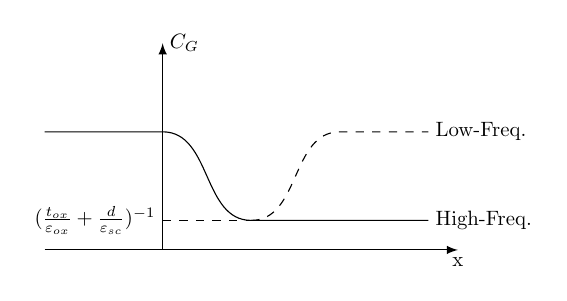
\begin{tikzpicture}[scale=0.75, transform shape]
        %asse x
        \draw[-latex](-2,0)--(5,0)node[below]{x};
        %asse y
        \draw[-latex](0,0)--(0,3.5)node[right]{$C_G$};

        %grafico
         \draw (-2,2)--(0,2) to [in=180, out=0] (1.5,0.5)--(4.5,0.5)node[right]{High-Freq.};
        \draw[dashed] (1.5,0.5) to [in=180, out=0] (3,2) --(4.5,2)node[right]{Low-Freq.};

        %label
        \draw   [dashed] (0,0.5)node[left]{$(\frac{t_{ox}}{\varepsilon_{ox}}+\frac{d}{\varepsilon_{sc}})^{-1}$}--(1.5,0.5);
    \end{tikzpicture}
    \caption{Caption}%
    \label{fig:enter-label}
\end{figure}


Viceversa, se il potenziale varia a frequenza moderata, si nota che la regione di svuotamento varia lentamente, quindi si formano nuove cariche $Q_n$ che abbassano la $C$ del MOS si abbassa per poi ritornare a quello di Cox. \\

L'accumulo di carica risulta molto dipendente dalla velocità con cui varia la tensione di gate, influenza sia la carica accumulata, quindi la capacità perchè la carica per muoversi lo fa più o meno velocemente. Un transistor NON funziona in continua ma solo in regione dinamica.\\
Tutto ciò è valido per un substrato P, per un di tipo N le considerazioni da fare sono duali.

\subsection{MOSFET} pg 512\\
Il MOSFET è un dispositivo molto diffuso, sopratutto in ambito digitale, perchè è caratterizzato da dimensioni compatte, elevata affidabilità ed ha un processo tecnologico relativamente semplice. \\
Il MOSFET è un transistore a effetto di campo in cui il canale conduttivo è formato principalmente dalla regione di inversione di una giunzione MOS. Pertanto l'elettrodo di controllo (il gate) agisce modulando elettricamente la concentrazione della carica mobile di canale. \\
Contrariamente al JFET in cui il canale varia il suo spessore ma la densità di carica libera resta circa costante, nel MOSFET il canale resta estremamente sottile e varia invece la concentrazione di carica libera presente in esso.
I MOSFET si dividono in due categorie principali, come gli altri FET: 
\begin{enumerate}
    \item MOSFET a canale n: lo strato di inversione è formato da elettroni, e il
substrato è di tipo p;
\item MOSFET a canale p: lo strato di inversione è formato da lacune, e il substrato
è di tipo n.
\end{enumerate}

Ciascuna delle due categorie precedenti si divide in due sottocategorie, dette MOSFET ad arricchimento e MOSFET a svuotamento .\\
Nei dispositivi ad arricchimento il canale conduttivo non esiste per Vgs <0,
ossia in tali condizioni il dispositivo è sotto soglia e Id = 0, ossia il MOSFET non
conduce, o è nello stato off, analogo ad un circuito aperto visto fra drain e source.\\

Nei dispositivi a svuotamento il canale conduttivo esiste per Vgs < 0, ossia in tali
condizioni il dispositivo conduce, o è on. Per portare sotto soglia il dispositivo a
svuotamento è necessario applicare al gate una tensione opportuna.\\
I dispositivi a svuotamento possono essere ottenuti variando opportunamente il drogaggio del canale, ossia ad esempio impiantando un sottile canale n in un substrato di tipo p (MOSFET a canale preformato). \\
In generale i MOSFET a canale n si comportano in modo simile ai FET a canale n per quanto riguarda le direzioni delle correnti e i segni delle tensioni di polarizzazione; i MOSFET a canale p sono analoghi aiFET a canale p.\\
Tipicamente il MOSFET è dotato di un quarto elettrodo, detto elettrodo di
bulk o di substrato, posto alla tensione Ves rispetto al source. Tale elettrodo permette di polarizzare il substrato e influisce sulle caratteristiche tensione-corrente
del dispositivo, in particolare sulla tensione di soglia. Il controllo della tensione di
soglia attraverso la polarizzazione del substrato, molto importante nei MOSFET
di prima generazione, è ora meno usato.
%
\cleardoublepage
%
\subsubsection{NMOS}
\subsection{Funzionamento di base}
Nel momento in cui $V_{GS}>0$  con Source e Bulk collegati a ground, si crea un campo elettrico idelmente uguale lungo tutto il gate e diretto verso il substrato. Le lacune vicino al substrato vengono allontanante mentre gli elettroni ne vengono attratti posizioniandosi il più vicino possibile lungo la superficie semiconduttore-ossido dove si ricombinano con le lacune in tale zona.

Aumentando $V_G$ oltre un certo valore di soglia, tutte le lacune in prossimità dell'ossido sono sparite, sia perchè si sono ricombinate sia perchè sono state spinte via.
Il numero di elettroni situati nella regione Ossido-Semiconduttore è aumentano a causa dell'inversione di popolazione (spiegato nel MOS), creando un canale sotto l'ossido e lungo $L_G$.\\
%
\begin{figure}[hbt!]
    \centering
    \includegraphics[width=0.45\textwidth]{Immagini/imm.9.11.2023/funzionamento mosfet.png}
    \caption{Caption}%
    \label{fig:enter-label}
\end{figure}
\\%
Ponendo $V_{DS}\neq 0$ con $V_S=0$, si determina un campo elettrico all'interno del canale lungo x e di conseguenza un potenziale $V_{ch}$. 
%
\begin{equation}
    V_{ch}(x)=-\int_{0}^{x}\mathcal{E}_{ch}(x')dx'
\end{equation}
%
Assumendo in prima approssimazione che il campo elettrico
lungo il canale sia costante (e pari a ${V_{th}}/{L_G}$), il potenziale risulterà crescere linearmente in funzione della posizione x partendo da 0 Volt sul Source fino a $V_D$ sul Drain.
%
\begin{figure}[hbt!]
    \centering
    \begin{tikzpicture}
        \node at (0,0.75)[anchor=south]{G};
        \draw (0,0.75)--(0,0.5);
        \draw[pattern = north east lines] (-2,0.5) rectangle ++(4,-0.2);
        \draw (-2,0.3) rectangle ++(4,-0.3);
        \draw[thick](-3,0)--++(6,0);
        \node at (-2,0.13)[right] {\scriptsize{$SiO_2$}};
        %disegno vettore potenziale
        \draw [-latex,blue](-1,-0.23)node[left]{$V_{ch}(x)$}--(1,-0.23);
        %disegno vettore campo
        \draw [-latex, red](1,-0.57)node[right]{$\mathcal{E}_x$}--(-1,-0.57);
        
        \begin{scope}[shift={(0,-0.3)}]
        % grafico
        \draw[-latex] (-2,-4) node[below]{0}--(2,-4)node[below]{$L_G$}--++(1,0)node[below]{$x$};
        \draw[-latex] (-2,-4) -- (-2,-1)node[right]{\textcolor{red}{$\mathcal{E}_X$} , \textcolor{blue}{$V_{CH}$}};
        %grafico rosso 
        \draw[red] (-2.3,-4) to [in=190, out= 45](-2,-3) -- (2,-3) to [in=135, out= -10](2.3,-4) ;
        %grafico blu 
        \draw[blue] (-2,-4)-- (2,-2) ;
        \draw[fill,blue] (2,-2) circle (0.5mm);
        \draw[dashed](-2,-2)--(2,-2);
        \draw[dashed](2,0.25)--(2,-4);
        \node at (-2,-2)[left]{$V_D$};
        \end{scope}
    \end{tikzpicture}
    \caption{Andamento del campo elettrico e della tensione di canale nel caso approssimato}
    \label{fig:Andamento del campo elettrico e della tensione di canale nel caso approssimato}
\end{figure}
\\%

\newpage
Il MOS mi ha fornito la legge di accumulo di carica $Q_n$ e vedo che l'equazione può essere adattata per descrivere anche l'accumulo di carica nel MOSFET:
%
\begin{equation}
    Q_n=-C_{ox}(V_G-V_{th})
\end{equation}
%
Questa formula mi stà dicendo che se $V_G=V_{th}$ non succede nulla mentre se $V_G>V_{th}$ si verifica l'inversione di popolazione.\\
%
\textbf{E' fondamentale capire che la soglia $V_{th}$, che $V_G$ dovrà superare affinchè si verifichi l'inversione di popolazione, non sarà più soltanto quel valore trovato nel MOS ($V_{th}=2\Phi_P$) ma ci sarà anche un nuovo contributo $V_{ch}$ creato dalla presenza del campo elettrico $\mathcal{E}_X$.\\}
Quindi $V_G > 2\Phi_P + V_{ch}$. Di solito, per stringere le equazioni si può scrivere che $V_{th}=2\Phi_P+V_{ch}$.\\

Se dopo tutte queste considerazioni inseriamo anche il potenziale di Bulk, si avrà la legge di controllo di carica nella seguente forma:
%
\begin{equation}
    Q_n = -C_{ox}(V_G-2\phi_P- V_{ch}) - \sqrt{2q\varepsilon_{} N_A(2\phi_P-V_B)}
\end{equation}
%
Un0altra osservazione interessante da fare è che la carica $Q_n$ che si forma lungo il canale $L_G$ varia in modo proporzionale a $V_{ch}$. La figura \ref{fig: Andamento dell'energia potenziale in un solido} mostra che la tensione di canale cambia linearmente in funzione di x, quindi anche la carica $Q_n$ lungo il canale ne sarà a sua volta dipendente.\\

Ulteriori osservazioni possono essere fatte fruttanto quello che ho detto nella sezione inerente alle non idealità del MOS.\\
%
\subsubsection{Calcolo della corrente in un MOSFET}
%
Riscrivo $Q_n$ usando il termine di Body Factor introdotto alla fine della sezione riguardante il MOS.
%
\begin{equation}
    Q_n=-C_{ox}(V_G-V_T-V_{ch})-\gamma_B C_{ox}[(2\Phi_P-V_B+V_{ch})^{1/2}-(2\Phi_P-V_B)^{1/2}]
\end{equation}
%
Dato un certo aumento della $V_G$, la presenza del canale fa sì che il massimo di $Q_n$ lo si abbia quando $V_{ch}$ risulta basso ($V_{ch}=0$), altrimenti l'incremento di $V_G$ viene mangiato dall'alto valore di $V_{ch}$ e quindi si introducono meno cariche all'interno del canale ($Q_n(L_G)>Q_n(0)$).\\

Per quello che ho descritto posso immaginare che vicino al source la quantità di cariche è molto maggiore rispetto alla quantità presente vicino al drain. In altre parole, \textbf{si ha un decremento di cariche avvicinandosi verso il drain.}
La figura \ref{fig:Forma del canale e andamento delle cariche} mi permette di capire subito che il canale così descritto, assume una forma trapezoidale.
%
\begin{figure}[hbt!]
    \centering
    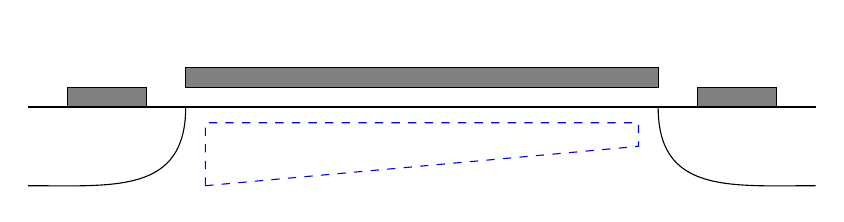
\begin{tikzpicture}
        \draw[white](0,0)--++(0,1); %lo metto spostare la figura più in basso. per dare spazio
        
        \draw(0,0)--(10,0);
        %metto metallizzazioni
        \draw[fill=gray](0.5,0)rectangle(1.5,0.25); %source
        \draw[fill=gray](2,0.25)rectangle(8,0.5); %gate
        \draw[fill=gray](8.5,0)rectangle(9.5,0.25); %drain
        %disegno zona source
        \draw(2,0)to[out=270, in=0,distance=1.1cm](0,-1);
        %disegno zona drain
        \draw(8,0)to[out=270, in=180,distance=1.1cm](10,-1);
        %disegno canale reale
        \draw[dashed,blue](2.25,-1)--(2.25,-0.2)--(7.75,-0.2)--(7.75,-0.5)--cycle;
    \end{tikzpicture}
    \caption{Forma del canale e andamento delle cariche}
    \label{fig:Forma del canale e andamento delle cariche}
\end{figure}\\
%
La Figura \ref{fig:Rappresentazione della forma del canale tramite modello con condensatori} è un modo comune per rappresentare il medesimo ragionamento sotto forma di un circuito equivalente costituito da tante capacità infinitesime poste in parallelo lungo tutto il canale $L_G$ (ricordare l'analogia MOS $\leftrightarrow$ condensatore).\\
\newpage
Ciascuna capacità è collegata tra il terminale di gate ed il terminale di canale $V_{ch}$. Immaginando che le capacità infinitesime abbiano un valore $C_i$ costante e sapendo che $V_{ch}$ è dipendente lungo x, arrivo a capire come la quantità di carica di un condensatore infinitesimo vari lungo la posizione infinitesima (dx) del canale:
%
\begin{equation}
    Q(x)=(C_1+C_2+...+C_N) \cdot \Delta V= C_{tot} \cdot (V_G-V_{ch}(x))
\end{equation}
%
\begin{figure}[hbt!]
    \centering
    \begin{circuitikz}
        \draw(0,0)--(10,0);
        
        %metto metallizzazioni
        %metallizzazione gate:
        \draw[fill=gray](2-0.25,1)rectangle(8+0.25,1.1);
        \draw (3.65+0.05+0.65*2,1+0.1)to[short]++(0,+0.25)node[above]{$V_G$};
        %source
        \draw[fill=gray](0.5-0.25,0)rectangle(1.5-0.25,0.25);
        %drain
        \draw[fill=gray](8.5+0.25,0)rectangle(9.5+0.25,0.25); 
        %metto le capacità
        \draw (2.35+0.05,1)to[C]++(0,-1)node[below]{$V_{ch1}$};
        \draw (3+0.05,1)to[C]++(0,-1)node[below]{$V_{ch2}$};
        \draw (3.65+0.05,1)to[C]++(0,-1);
        \draw (3.65+0.05+0.65,1)to[C]++(0,-1);
        \draw (3.65+0.05+0.65*2,1)to[C]++(0,-1);
        \draw (3.65+0.05+0.65*3,1)to[C]++(0,-1);
        \draw (3.65+0.05+0.65*4,1)to[C]++(0,-1);
        \draw (3.65+0.05+0.65*5,1)to[C]++(0,-1);
        \draw (3.65+0.05+0.65*6,1)to[C]++(0,-1)node[below]{$V_{chn}$};
        
        %disegno substrato source
        \draw(2-0.25,0)to[out=270, in=0,distance=1.1cm](0,-1);
        %disegno substrato drain
        \draw(8+0.25,0)to[out=270, in=180,distance=1.1cm](10,-1);
    
        %Qch
        \begin{scope}[shift={(0,-0.6-2.25)},yscale=-1]
            \draw[-latex](2,-2.2)--(8,-2.2)node[anchor= west]{$x$};;
            \draw[-latex](2,-2.2)--(2,-0.6)node[right,blue]{$Q_{ch}$ and channel form};
            \draw [pattern color=blue,pattern=north east lines](2.25,-1.5+0.25)--(7.75,-2.2+0.25)--++(0,-0.24)--(2.25,-2.2)--(2.25,-1.5+0.25);
        \end{scope}
        %Vch
        \begin{scope}[shift={(0,-2.4)}]
            \draw[-latex](2,-2.2)--(8,-2.2)node[right]{$x=L_G$};;
            \draw[-latex](2,-2.2)--(2,-0.6)node[right]{$V_{ch}$};
            \draw (2.25,-2.2)--(7.75,-1.5);
            \draw [densely dashed](7.75,-1.5)--(7.75,-2.2);
            \draw [densely dashed] (7.75,-1.5)--(2,-1.5)node[left]{$V_D$};
        \end{scope}
    \end{circuitikz}
    \caption{Rappresentazione della forma del canale tramite modello con condensatori}
    \label{fig:Rappresentazione della forma del canale tramite modello con condensatori}
\end{figure}
\\%
A partire da queste considerazioni si può scrivere la corrente che scorre tra Drain e Source in funzione di x:
%
\begin{equation*}
    I_{ds}(x)=W \cdot J_{ds}(x)=-W\cdot \mu_n\ Q_n(V_G,V_B,V_{ch})\ \mathcal{E}=
\end{equation*}
%
\begin{equation}
    I_{ds}=-W\ \mu_n\ Q_n(V_G,V_B,V_{ch})\cdot \dfrac{dV_{ch}}{dx}
\end{equation}
Dove $W$ è la profondità del transistor. 
Allora:
\begin{equation}
    \int_{0}^{L_G}I_{DS}(x) \ dx =\int_{V_{ch}(0)}^{V_{ch}(L_G)}-W\ \mu_n\ Q_n(V_G,V_B;V_{ch})\ dV_{ch}
\end{equation}
Ma la corrente $I_{ds}$ che attraversa il canale di un MOSFET deve essere costante lungo tutto il canale per rispettare la legge di continuità. Questo significa che la quantità di carica che entra nel canale deve essere uguale a quella che esce, altrimenti ci sarebbe un accumulo di carica, che non è fisicamente possibile in uno stato stazionario.\\
Per questo motivo devo imporre la condizione $I_{ds}(x) = cost = I_{ds}$, ottenendo:
%
\begin{equation*}
    I_{ds} \cdot L_G=W\ \mu_n \int_{V_{ch}(0)=0V}^{V_{ch}(L_G)=V_{DS}} Q_n(V_{ch})\ dV_{ch}
\end{equation*}
%
lo riscrivo (qui tolgo il meno, in realtà c'è ancora)
%
\begin{equation}
    I_{ds}=\dfrac{W\ \mu_n}{L_G} \int_{V_{ch}(0)=0V}^{V_{ch}(L_G)=V_{DS}} Q_n(V_{ch})\ dV_{ch}
\end{equation}
%
sostituendo l'espressione di $Q_n$ ottengo:
%
\begin{equation}
    I_{ds}=\dfrac{W\ \mu_n\ C_{ox}}{L_G} \left[\int_{0}^{V_{ds}} (V_{gs}-V_{ch}-V_T)dV_{ch}-\gamma_B \ \int_{0}^{V_{ds}}[(2\Phi_P-V_B+V_{ch})^{1/2}-(2\Phi_P-V_B)^{1/2}]\  dV_{ch}\right]
\end{equation}
%
il risultato è :
%
\begin{equation}
    I_{ds}= \dfrac{W\ \mu_n\ C_{ox}}{L_G}\left[ (V_{gs}-V_T)V_{ds}-\dfrac{1}{2}V_{ds}^2\right]-\gamma_B \left[ \dfrac{2}{3}[(2\Phi_P-V_B+V_{ch})^{3/2}-(2\Phi_P-V_B)^{3/2}]-(2\Phi_P-V_{B})^{1/2}V_{ds}\right]
\end{equation}
%
Se $\gamma_B \ll 1$ allora l'espressione può essere approssimata:
%
\begin{equation}
    I_{ds}= \dfrac{W\ \mu_n\ C_{ox}}{L_G}\left[ (V_{gs}-V_T)V_{ds}-\dfrac{1}{2}V_{ds}^2 \right]
\end{equation}
%
E' importante ricordare che l'espressione calcolata non è altro che un modello matematico e come tale va preso con attenzione. In particolare non ha senso considerare i casi in cui $V_G-V_T-V_{ch} <0$ perchè altrimenti la corrente cambierebbe di segno. L'unica variabile che varia è $V_{ch}$, quindi sarebbe da interpretare come una corrente che cambia verso all'aumentare della tensione di canale,cosa che non ha senso in questo contesto.
Quello che realmente succede al crescere della tensione di canale è spiegata nella seguente Figura:

\begin{figure}[htp!]
\centering
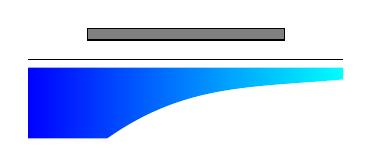
\begin{tikzpicture}
    \draw[fill=gray](-1.25,0.25) rectangle++(2.5,0.15);
    \draw(-2,0) -- (2,0);
    
    % Disegno della popolazione di elettroni con un gradiente da blu a ciano
    \shade[left color=blue,middle color= blue!50, right color=cyan] 
    (-2,-0.1) -- ++(4,0) -- ++(0,-0.15) to [in=35, out=185] (-1,-1) -- ++(-1,0) -- ++(0,0.9) -- cycle;


\end{tikzpicture}
\hspace{1cm}
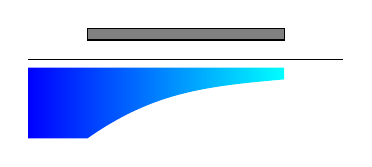
\begin{tikzpicture}
    % Disegno della prima figura con gradiente da blu a ciano
    \shade[left color=blue, middle color=blue!50, right color=cyan]
    (-2,-0.1) -- ++(3.25,0) -- ++(0,-0.15) to [in=35, out=185] (-1.25,-1) -- ++(-0.75,0) -- ++(0,0.9) -- cycle;
    
    % Disegno della barra grigia sopra
    \draw[fill=gray] (-1.25,0.25) rectangle ++(2.5,0.15);
    
    % Linea orizzontale
    \draw (-2,0) -- (2,0);
\end{tikzpicture}
\hspace{1cm}
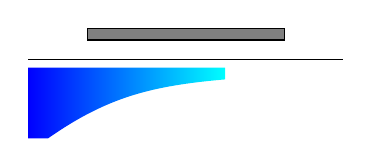
\begin{tikzpicture}
    % Disegno della seconda figura con gradiente da blu a ciano
    \shade[left color=blue, middle color=blue!50, right color=cyan]
    (-2,-0.1) -- ++(2.5,0) -- ++(0,-0.15) to [in=35, out=185] (-1.75,-1) -- ++(-0.25,0) -- ++(0,0.9) -- cycle;
    
    % Disegno della barra grigia sopra
    \draw[fill=gray] (-1.25,0.25) rectangle ++(2.5,0.15);
    
    % Linea orizzontale
    \draw (-2,0) -- (2,0);
\end{tikzpicture}


\caption{Forma del canale al variare di $V_D$}
\label{fig:Forma del canale al variare di $V_D$}

\end{figure}


per spiegare il comportamo della figura considero il caso standard Figura \ref{Forma del canale al variare di $V_D$}, mostrata a sinistra.
In questo caso , come visto prima, la sezione della regione di svuotamento ha sezioene (circa) trapezoidale con un restringimento verso il drain. laddove $V_{G}-V_{T}=V_D$ il canale si "annulla" e l'estremo destro del canale ha carica zero ($Q_n(L_G)=0$).\\
$ES:se V_G-V_T=4V, V_D=4V,$ \\

Qualora $V_D>V_{DSS}$, il canale inizia a ridursi un un punto $x'$ prima della fine della lunghezza $L_G$, ovvero $Q_n(x'<L_G)=0$.\\
Maggiore è $V_D$, maggiore sarà la carica spaziale rimossa.

Questo significa che ci sarà un $x'$ per il quale $V_{ch}(x')=V_G-V_T$ dove, per $x<x'$ ci sarà ancora carica mentre per $x>x'$, la carica è nulla.\\

Questo fenomeno non è contemplato nell'equazione della continuità di corrente perciò la validità di queste assunzioni è mantenuta solo entro il limite posto dalla condizione $V_{ch} (L_G)=V_{DS} \leq V_{gs}-V_{th}$.\\

Per il teorema matematico di Fermat, il massimo della corrente si trova ponendo la derivata della corrente rispetto alla tensione $V_{ds}$:
%
\begin{equation}
    \dfrac{dI_{ds}}{dV_{ds}}=0
\end{equation}
%
Da questo trovo che il massimo di corrente si ha nel punto in cui $V_{ds}=V_G-V_{th}$. Allora la corrente massima vale:
%
\begin{equation}
    I_{ds}^{max}=I_{ds}^{sat}\dfrac{W\ \mu_n\ C_{ox}}{2\ L_G}(V_G-V_{th})^2
\end{equation}
%
equazione valida per $V_D \geq V_G-V_{th}$.\\
\newpage
Se scrivo l'andamento della $I_{DS}$ in funzione di $V_{DS}$ ottengo la caratteristica I-V del MOSFET:
%
\begin{figure}[hbt!]
    \centering
    
\includegraphics[width=1\textwidth]{ImmaginiMOS/mos caratteristica.png}
    \caption{Caratteristica I-V del MOSFET}
    \label{fig:Caratteristica I-V del MOSFET}
\end{figure}
\\%
Il canale si estingue ad una coordinata che dipende da $V_G-V_{th}$, per quella particolare situazione la corrente è stabilita dall'integrale visto in precedenza. L'assenza di carica impedirebbe il passagio di corrente per $\forall x > x'$ t.c. $V_{ch}(x)>V_{DSS}$.\\
Nella realtà succede un fenomeno di strozzamento visibile nel diagramma a bande.\\

Per la continuità della corrente, se c'è un certo valore di corrente in una sezioni qualsiasi del canale, allora queste non possono cessare bruscamente nella sezione successiva.\\
La $I_{ds}^{sat}$ raggiungerà valori sampre più alti al crescere di $V_G$, NON si ha quindi dipendenza da $V_D$ in prima approssimazione.\\
un modello matematico della corrente che risulta più corretto è:
%
\begin{equation}
    I_{ds}^{sat}=\dfrac{W\ \mu_n\ C_{ox}}{2L_G}(V_G-V_{th})^2 \cdot (1+\lambda V_{ds})
\end{equation}
%
Il termine $\lambda$ tiene conto del restringimento che subisce il canale all'aumentare di $V_{ds}$ che comporterà la diminuzione di $I_{ds}$.\\

Un modello circuitale che descrive, in prima approssimazione, il comportamento del MOSFET è descritto in Figura \ref{fig:Modello in prima approssimazione del MOSFET}.
Il transistor in saturazione si comporta come un condensatore (che disaccoppia la continua) quando lo si guarda verso l'ingresso e si comporta da generatore di corrente quando lo si guarda verso l'uscita
%
\begin{figure}[hbt!]
    \centering
    \begin{circuitikz}
        \draw(0,0)node[left]{S} to [short,*-](2,0) coordinate (gndGS) --(4,0) coordinate (gndDS) to [short](6,0)node[right]{S};
        \draw (0,2)node[left]{G} to [short,*-]++(2,0) to [C,l_=$C_{ox} \approx$,-*](gndGS);
        \draw (6,2)node[right]{D} to [short,*-]++(-2,0) to [I,invert,l=$?$,-*](gndDS);
        
    \end{circuitikz}
    \caption{Modello in prima approssimazione del MOSFET}
    \label{fig:Modello in prima approssimazione del MOSFET}
\end{figure}
\\%
\cleardoublepage
%
\subsubsection{Approssimazione del gate come una capacità}
Dato l'andamento del canale a forma trapezoidale, scrivo:
\begin{equation}
    Q_n(x)=-C_{ox}[V_G-V_T-V_{ch}(x)]
\end{equation}
se voglio calcolare la carica totale nel caso monodimensionale, nella sola direzione delle x:
\begin{equation}
    Q_{nx}^{tot}=\int_{0}^{L}Q_n(x)\ dx
\end{equation}
Se invece lo calcolo in tutte le direzioni (x,y):
\begin{equation}
    Q_{nxy}^{tot}=\int_{0}^{L}\int_{0}^{W} Q_n(x)\ dx
\end{equation}
Ora posso definire una corrente di gate:
\begin{equation}
    I_{gs}(x)=\dfrac{dQ_n^{tot}}{dt}=C_{gs}\dfrac{dV_{GS}}{dt}
\end{equation}
L'ultima uguaglianza è valida solo nell'ipotesi in cui il mosfet stia operando nell'intorno del punto di lavoro, quando il canale non modofica troppo la forma.\\
ecco perchè nel modello precedente vedo che l'ingresso del gate è praticamente un condensatore.

\section*{13.11.2023}
\subsubsection{Campo elettrico non costante}
Sia  $I_{ds}=\dfrac{\mu_n\ C_{ox}\ W}{L_G}\left[ (V_{gs}-V_{th})V_{ds}-\dfrac{1}{2}V_{ds}^2\right]$ la corrente che misuro. Posso pensare di prendere la corrente $I_{ds}$ che scorre lungo una generica sezione del canale. per fare questo riscrivo l'equazione rappresentandola in funzione di $x$ t.c $0<x<L_G$ :
%
\begin{equation}
    I_{ds}(x)=I_{ds}=\dfrac{\mu_n\ C_{ox}\ W}{\textcolor{red}{x}}\left[ (V_{gs}-V_{th})\textcolor{red}{V_{ch}}-\dfrac{1}{2}\textcolor{red}{V_{ch}}^2\right]
\end{equation}
%
Dove ho posto $ I_{ds}(x)=I_{ds}$ perchè ricordo che la corrente è costante in tutte le sezioni.\\
Poi considero il punto in cui il canale si stringe molto e la corrente raggiunge la saturazione. In questo caso l'andamento della $I_{ds}$ è :
%
\begin{equation}
    I_{ds}=\dfrac{\mu_n\ C_{ox}\ W}{2L_G}(V_{gs}-V_{th})^2
\end{equation}
%
Siccome, però, la corrente è uguale sezione per sezione allora $I_{ds}^{sat}=I_{ds}(x)$. Quindi posso riscrivere:
%
\begin{equation}
    \dfrac{\mu_n\ C_{ox}\ W}{2L_G}(V_{gs}-V_{th})^2=\dfrac{\mu_n\ C_{ox}\ W}{x}\left[ (V_{gs}-V_{th})V_{ch}-\dfrac{1}{2}V_{ch}^2\right]
\end{equation}
%
Questa è un'equazione di secondo ordine e come tale avrà due soluzioni possibili. Risolvendolo si vedrà che una delle due, in realtà, è una soluzione non fisica perciò l'unico risultato risulta essere:
%
\begin{equation}
    V_{ch}(x)=(V_{gs}-V{th})\left( 1-\sqrt{1-\dfrac{x}{L_G}}\right)
\end{equation}
%
Per capire meglio il significato di questo risultato vado a graficare l'andamento ideale e la confronto con il risultato reale:
%
\begin{figure}[hbt!]
    \centering
    \begin{tikzpicture}
        \draw[-latex](0,0)--++(5,0)node[right]{x};
        \draw[-latex](0,0)--++(0,2.5)node [left]{$\dfrac{V_{ch}}{(V_{GS}-V_{th})}$};
        %disegno grafico reale
        \draw(0,0)--(4.5,2);
        %disegno grafico reale;
        \draw[red](0,0) to [out=0, in=250](4.5,2);
        %tratteggi e label
        \draw[dashed](4.5,2)--(0,2)node[left]{$1$};
        \draw[dashed](4.5,2)--(4.5,0)node[below]{$L_G$};
    \end{tikzpicture}
    \caption{Tensione del canale normalizzata con andamento ideale (nero) VS reale (rosso)}
    \label{fig:enter-label}
\end{figure}
\\%
Capisco che l'andamento del potenziale lungo il canale non è lineare e di conseguenza non posso più dire che il campo elettrico sia costante. In particolare, 
 $\mathcal{E}$ assume un valore massimo vicino alla zona di Drain ($\approx L_G$) e questo lo si spiega ricordando la teoria del pinch-off e la formula della corrente nel canale:
Lo spessore del canale si riduce avvicinandosi verso il Drain con la conseguente diminuzione di elettroni ($n\downarrow$) , allora mi dovrei aspettare che la corrente diminuisca. Dopotutto avevo considerato $\mathcal{E}=cost$ pertanto:
%
\begin{equation}
    I_{ds}=W\ q\ n\ \mu_n \mathcal{E} \Rightarrow \text{se } n\downarrow \text{allora } I_{ds}\downarrow
\end{equation}
%
In realtà so che, per la continuità della corrente, $I_{ds}$ rimane costante sezione per sezione e affinchè questo avvenga è necessario che un'altro parametro compensi la diminuzione di elettroni. Ecco spiegato il motivo del perchè il campo elettrico è massimo in prossimità del Drain: perchè \textbf{in prossimità del Drain la concentrazione di elettroni è minore}.\\

\subsubsection{Breakdown MOSFET}
La diretta conseguenza di avere un elevato campo elettrico nella zona di Drain riguarda il fatto che la regione di svuotamento nel suo intorno risulta essere molto "stressata" e questo mi porta a pensare a tutta la teoria riguardante il breakdown.\\
per capire meglio posso guardare la figura seguente:
%
\begin{figure}[hbt!]
    \centering
    \begin{circuitikz}
        \draw (0,0)--++(6,0);
        \draw (0,-2)--++(6,0);
        \node at (0.15,-1.75){p};
        %regione svuotata n+ drain e label
        \draw(6,-1) to [out=180, in=270,distance=1cm](6-1.5,0);
        \node at (5.45,-0.5)[]{n+};
        %regione svuotata n+ source e label
        \draw(0,-1) to [out=0, in=270,distance=1cm](0+1.5,0);
        \node at (0.85,-0.5)[]{n+};
        %canale
         \draw(0.15+1.5,-0.07)--++(2.8,0)--++(-2.825,-0.5)--cycle;
        %regione di svuotamento zona drain 
         \draw[dashed, red](6,-0.9) to [out=180, in=270,distance=1cm](6-1.4,0);
         %regione di svuotamento zona source 
         \draw[dashed, red](0,-0.9) to [out=0, in=270,distance=1cm](1.4,0);
         
         %regione svuotata
         \draw[dashed, blue](0,-1.3)to[out=0, in=270](1.6,-0.6)--(0+3,-0.6)--(1+3,-0.6)to[out=270, in=180](3+3,-1.75);

        %metallizzazione gate
        \draw[fill=lightgray](1.5,0.5)rectangle(6-1.5,0.6);
        \draw (3,0.6)to[short]++(0,+0.15)node[above]{$V_G>V_{th}$};
        
        %metallizzazione drain
        \draw[fill=lightgray](6-1.5,0)rectangle(6,0.1);
        \draw (6-1.5+0.75,0.1)to[short]++(0,+0.15)node[above]{$V_D>0$};
        %metallizzazione source
        \draw[fill=lightgray](3-1.5,0)rectangle(0,0.1);
        \draw (0.75,0.1)to[short]++(0,+0.15)node[above]{$V_S=0$};
        %metallizzazione bulk
        \draw[fill=lightgray](0,-2)rectangle(6,-2-0.1);
        \draw (3,-2.1) to[short] ++(0,-0.3) node[tlground]{};
        \node[right] at (3.1,-2-0.3) {$V_B = 0$};
        %diodo
        \draw (5.75,-2) to [D,*-*]++(0,+1.4);
    \end{circuitikz}
    \caption{Regione di svuotamento nella condizione di inversione di popolazione}
    \label{fig:Regione di svuotamento nella condizione di inversione di popolazione}
\end{figure}
\\%
Il canale costituito da elettroni è collegato alla zona di drain. La giunzione tra drain e semiconduttore P crea un regione di svuotamento piuttosto grande, sufficiente a piegare le bande talmente tanto da permettere il passaggio degli elettroni per effetto tunnel.\\
Voglio quindi valutare il massimo campo elettrico sopportabile dal MOSFET in modo da prevenire l'effetto breakdown nella zona più a rischio. Per fare questo considero la regione di svuotamento che si verifica nella giounzione semiconduttore P-Drain e la tratto esattamente come farei per una giunzione pn+.\\
Siccome il drain è fortemente drogato ($N_D\gg N_A$, da cui $N_{eq}=1/N_A$) allora la regione di svuotamento si estenderà maggiormente lungo il substrato P.\\
Posso quindi fare un'approssimazione e considerare la regione di svuotamento solo lungo il semiconduttore P. Da qui si capisce come mai  lo spessore della regione svuotata $\left(x_p=\sqrt{\dfrac{2\ \varepsilon_{sc} \ (V_{bi}-V_{A})}{q\ N_A}\dfrac{1}{N_A}}, \text{ con } \ V_A=V_D-V_B\right)$ ha una banda così sottile da  permettere il breakdown.\\

Per il teorema di Gauss il campo elettrico totale risulta essere:
\begin{equation}
    \mathcal{E}_{max}=q\dfrac{N_Ax_p}{\varepsilon_{sc}}=\sqrt{\dfrac{2qN_AV_{DS}}{\varepsilon_{sc}}}
\end{equation}
\begin{ricevimento}
    non mi tornano le formule
\end{ricevimento}
La soluzione a questo problema è ridurre l'estensione della regione svuotata 
realizzando un nuovo pozzetto drogato n, tra il canale ed il Drain drogato n+, portando alla creazione dei cosiddetti MOS lateralmente diffusi.
%
\begin{figure}[hbt!]
    \centering
    \begin{circuitikz}
        \draw (0,0)--++(6+1.4,0);
        \draw (0,-2)--++(6+1.4,0);
        \node at (0.15,-1.75){p};
        %drogaggio n drain e label
        \draw(6+1.4-1.4,-0.65) to [out=180, in=270,distance=0.6cm](6+1.4-1.5-0.75,0);
        \node at (5.65,-0.3)[]{n};
        %drogaggio n+ drain e label
        \draw(6+1.4,-1) to [out=180, in=270,distance=1cm](6+1.4-1.5,0);
        \node at (5.45+1.4,-0.5)[]{n+};
        %drogaggio n+ source e label
        \draw(0,-1) to [out=0, in=270,distance=1cm](0+1.5,0);
        \node at (0.85,-0.5)[]{n+};
        %canale
         \draw(0.15+1.5,-0.07)--++(2.8+0.7,0)--++(-2.825-0.7,-0.5)--cycle;
        %regione di svuotamento zona drain n+
         \draw[dashed, red](6+1.4,-0.9) to [out=180, in=300,distance=0.5cm](6+1.4-1.3,-0.55);
          %regione di svuotamento zona drain n
         \draw[dashed, red](6+1.4-1.3,-0.45) to [out=180, in=270,distance=0.5cm](6+1.4-2,0);
         %regione di svuotamento zona source 
         \draw[dashed, red](0,-0.9) to [out=0, in=270,distance=1cm](1.4,0);
         
         %regione svuotata
         \draw[dashed, blue](0,-1.3)to[out=0, in=270](1.6,-0.6)--(0+3+1.4,-0.6)--(1+3+1.1,-0.6)to[out=270, in=180](5+0.8,-0.9)to[out=270, in=180](3+3+1.4,-1.75);;

        %metallizzazione gate
        \draw[fill=lightgray](1.5,0.5)rectangle(6+0.7-1.5,0.6);
        \draw (3+0.35,0.6)to[short]++(0,+0.15)node[above]{$V_G>V_{th}$};
        
        %metallizzazione drain
        \draw[fill=lightgray](6+0.65-1.5,0)rectangle(6+1.4,0.1);
        \draw (6+1.4-1.5+0.75,0.1)to[short]++(0,+0.15)node[above]{$V_D>0$};
        %metallizzazione source
        \draw[fill=lightgray](3-1.5,0)rectangle(0,0.1);
        \draw (0.75,0.1)to[short]++(0,+0.15)node[above]{$V_S=0$};
        %metallizzazione bulk
        \draw[fill=lightgray](0,-2)rectangle(6+1.4,-2-0.1);
        \draw (3+0.7,-2.1) to[short] ++(0,-0.3) node[tlground]{};
        \node[right] at (3.1+0.7,-2-0.3) {$V_B = 0$};
        
    \end{circuitikz}
    \caption{Regione di svuotamento nella condizione di inversione di popolazione con pozza n}
    \label{fig:Regione di svuotamento nella condizione di inversione di popolazione con pozza n}
\end{figure}
\\%
In questa configurazione, l'estremità del canale (costituito dal campo elettrico massimo) tocca una giuzione pn e quindi la regione di svuotamento si estende in maniera equa sia nella regione n che p
\begin{exbox}
    ricordare che le dimensione delle regioni di svuotamento devono sostare alla regola:
    \begin{equation*}
        N_A|x_p|=N_d |x_n|
    \end{equation*}
    Da cuicapisco che se $N_D > N_A$ allora xp cresce per rispettare l'uguaglianza.
    \begin{equation*}
        |x_p|=\dfrac{N_D}{N_A} |x_n|
    \end{equation*}
\end{exbox}
L'espressione del campo elettrico risulta:
\begin{equation}
    \mathcal{E}_{max}=\dfrac{q}{\varepsilon_{sc}}\sqrt{\dfrac{2qV_{DS}}{\varepsilon_{s}}\cdot \dfrac{N_D}{1+\dfrac{N_D}{N_A}}}
\end{equation}
\begin{ricevimento}
    non mi tornano le formule inoltre vbi-va=vds??
\end{ricevimento}
notare dall'equazione come all'aumentare di $N_D$, l'espressione del campo torna ad essere uguale a quello del caso precedente. Viceversa, al diminuire di $N_D$ è possibile utilizzare il mosfet per $V_{DS}$ maggiori per raggiungere lo stesso campo elettrico. 
(di ciò ne risente anche la capacità (??)
\subsubsection{Effetto sulla carica}
voglio calcolare la carica totale:
\begin{align}
    Q_n^{tot}&=W\int_{0}^{L_G} C_{ox}\left[ (V_{gs}-V_T)-\underbrace{(V_{gs}-V_{th})\left( 1-\sqrt{1-\dfrac{x}{L_G}}\right)}_{V_{ch}(x)}\right] dx \\
    &=\dfrac{2}{3}\ W\ L_G\ C_{ox}(V_{gs}-V_T)
\end{align}
%
\begin{figure}[hbt!]
    \centering
    \begin{tikzpicture}
        \draw[fill={rgb:black,6;white,5}] (0,0)--(3,0)--(3,0.5)--(0,0.5)--(0,0);
        \draw[fill={rgb:black,4;white,7}] (0,0.5)--(3,0.5)--(5,1.5)--(2,1.5)--(0,0.5);
        \draw[pattern=north east lines, pattern color=black] (3,0)--(3,0.5)--(5,1.5)--(5,1)--(3,0); 
       \draw[pattern=north east lines, pattern color=black] (-3,-0.5)--(3.5,-0.5)--(7.5,1.5)--(1,1.5)--(-3,-0.5); 
       %frecce e label
       \draw[latex-latex](2,1.75)--(5,1.75)node[pos=.5,above]{$L_G$};
       \draw[latex-latex](4,-0.5)--(8,1.5)node[pos=.5, below right ]{$W$};
    \end{tikzpicture}
    \caption{Caption}%
    \label{fig:enter-label}
\end{figure}
\\%
\newpage
Ora posso calcolare la capacità $C_{gs}$ dalla variazione di carica totale rispetto al potenziale applicato, trovando:
%
\begin{equation}
    C_{gs}=\dfrac{2}{3}WLC_{ox}
\end{equation}
%
Il modello del MOSFET diventa il seguente:
%
\begin{figure}[hbt!]
    \centering
    \begin{circuitikz}
        \draw(0,0)node[left]{S} to [short,*-](2,0) coordinate (gndGS) --(4,0) coordinate (gndDS) to [short,-*](6,0)node[right]{S};
        \draw (0,2)node[left]{G} to [short,*-]++(2,0) to [C,l_=$\frac{2}{3}WLC_{ox}$,-*](gndGS);
        \draw (6,2)node[right]{D} to [short,*-]++(-2,0) to [I,l=$\frac{\mu_nC_{ox}W}{2L_G}(V_{GS}-V_{th})^2$,-*](gndDS);
        
    \end{circuitikz}
    \caption{Caption}%
    \label{fig:enter-label}
\end{figure}
\\%
Posso calcolare il tempo di transito $\tau_t$ che ha senso solo nella condizione di saturazione (??).
Facendo le dovute sostituzioni si ha
%
\begin{equation}
    \tau_T=\dfrac{4}{3} \dfrac{L_g^2}{\mu_n (V_{GS}-V_T)}
\end{equation}
%
ora, dato il tempo di transito posso pensare anche di introdurre il concetto di frequenza di transito che sarà la massima frequenza di funzionamento.
Il fatto che tale frequenza sia dipendente dal tempo di transito ($f_t^{max}(\tau_t)$) e che il tempo di transito sia dipendente dalla polarizzazione del gate, mi porta a dire anche che anche la frequenza sia dipendente da ($V_{GS}-V_T$).

\paragraph{Calcolo della frequenza massima di funzionamento. Il prodotto guadagno banda}\mbox{}\\

Come nel caso del BJT, vorrei studiare il caso in cui si ottiene massima corrente in uscita.\\
Considero quindi il caso di uscita in cortocircuito poichè è la condizione necessaria per ottenere il massimo guadagno di corrente.
La frequenza alla quale corrisponde il guadagno unitario corrisponde alla $f_{taglio}$.

la Current gain in CC:
$A_I^{CC}(\omega)=A^{CC}(2\pi f \tau)=1$
Prendo il modello della figura precedente e ne cortocircuito il carico. Successivamente calcolo la corrente di ingresso e di uscita:
%
\begin{equation}
    I_{in}(\omega)=\dfrac{V_{gs}}{Z_{gs}}=\omega\ C_{gs}\ V_{gs}
\end{equation}
%
\begin{equation}
    I_{out}(\omega)=-\frac{\mu_nC_{ox}W}{2L_G}(V_{GS}-V_{th})^2=g_m \cdot V_{gs}
\end{equation}
dove la conduttanza vale $g_m=\frac{\mu_nC_{ox}W}{2L_G}(V_{G}-V_{th})$.\\
%

in generale, il guadagno di corrente si può trovare facendo il rapporto tra $|I_{in}(\omega)|$ e $|I_{out}(V_g)|$. Quindi si troverà che:
%
\begin{equation}
    A_I^{CC}(\omega)=\dfrac{g_m V_{gs}}{\omega C_{gs} V_{gs}}
\end{equation}
%
Siccome il guadagno di corrente in cortocircuito deve essere unitario:
%
\begin{equation}
    \dfrac{g_m}{\omega C_{gs}}=1
\end{equation}
%
da cui
%
\begin{equation}
    f_t=\dfrac{g_m}{2\pi C_{gs}}=\dfrac{1}{\pi}\dfrac{3}{4}\dfrac{\mu_n (V_G-V_T)}{L_g^2} = \dfrac{1}{\pi \tau_t}
\end{equation}


\begin{exbox}
    The MOS transistor is a voltage controlled current source with the emphasis on current source. In order to produce an AC current at the output another AC current at the input is required to drive the gate. The gate is mainly a capacitive load and therefore the current to drive it increases with increasing frequency.

The frequency where the input current equals the output current is called the transition frequency. Above this frequency the transistor needs more current to be driven than it generates, it's useless.

The transition frequency depends on the parasitics and therefore on the technology. It is an important figure-of-merit that increases with smaller technologies.
\\
--------------------------------------------------------\\
Il gate di un MOSFET è essenzialmente un condensatore. Ricorda che se una tensione CA (V) a frequenza (f) viene immessa in un condensatore (C), la corrente risultante (I) è..

I = V * 2 * pi * f * C

Nota anche che l'uscita di un MOSFET è una corrente. 
La frequenza di guadagno unitario è importante perché definisce la frequenza, al di sopra della quale, devi immettere più corrente CA nel gate di quanta ne otterrai in uscita. 
Pertanto, definisce la frequenza utile massima per quel transistor se vuoi ottenere un'amplificazione in termini di corrente CA in ingresso rispetto a corrente CA in uscita.

Ad esempio, se avessi un MOSFET con una frequenza di guadagno unitario di 100 MHz, non potresti usarlo per amplificare un segnale da 1 GHz.

Inoltre, supponiamo di avere un circuito costituito da più MOSFET dello stesso tipo (come la maggior parte dei circuiti integrati) in cui l'uscita (drain) di un MOSFET viene utilizzata per pilotare l'ingresso (gate) di un altro MOSFET. Otterremo un'amplificazione del segnale solo se riusciremo a ottenere più corrente dal MOSFET di quanta ne immettiamo. Quindi, se stessimo costruendo amplificatori o circuiti digitali da MOSFET, la frequenza di guadagno unitario fungerebbe da limite massimo sulla frequenza operativa del circuito.

\end{exbox}
%
\cleardoublepage
